%%%%%%%%%%%%%%%%%%%%%%%%%%%%%%%%%%%%%%%%%%%%%%%%%%%%%%%%%%%%%%%%%%%%%%%%%%%%%%%%
% FUENTE
%%%%%%%%%%%%%%%%%%%%%%%%%%%%%%%%%%%%%%%%%%%%%%%%%%%%%%%%%%%%%%%%%%%%%%%%%%%%%%%%

% Plantilla creada por Eduardo Mosqueira Rey a partir de un original de
% Rational Software Corporation

%%%%%%%%%%%%%%%%%%%%%%%%%%%%%%%%%%%%%%%%%%%%%%%%%%%%%%%%%%%%%%%%%%%%%%%%%%%%%%%%
% CONFIGURACIÓN TEXSTUDIO DEL CORRECTOR ORTOGRÁFICO
%%%%%%%%%%%%%%%%%%%%%%%%%%%%%%%%%%%%%%%%%%%%%%%%%%%%%%%%%%%%%%%%%%%%%%%%%%%%%%%%

% !TeX spellcheck = es_ES
% Usar el lenguaje es_ES para la corrección en castellano

%%%%%%%%%%%%%%%%%%%%%%%%%%%%%%%%%%%%%%%%%%%%%%%%%%%%%%%%%%%%%%%%%%%%%%%%%%%%%%%%
% TIPO DE DOCUMENTO Y PAQUETES
%%%%%%%%%%%%%%%%%%%%%%%%%%%%%%%%%%%%%%%%%%%%%%%%%%%%%%%%%%%%%%%%%%%%%%%%%%%%%%%%

\documentclass[12pt, a4paper, titlepage]{article}

\usepackage[spanish]{babel} % Soporte multilenguaje para LaTeX.
\usepackage[a4paper, top=2.5cm, bottom=2.5cm, left=2.5cm, right=2.5cm]{geometry} % Interfaz flexible para definir las dimensiones del documento
\usepackage[utf8]{inputenc} % Aceptar diferentes tipos de codificación de caracteres de entrada (en este caso usamos la codificación Unicode UTF-8)
\usepackage{graphicx} % Soporte aumentado para gráficos 
\usepackage{color} % Para usar colores
\usepackage{hyperref} % Para manejar referencias cruzadas. P.ej. añadir hiperenlaces al índice


\begin{document}
	
	%%%%%%%%%%%%%%%%%%%%%%%%%%%%%%%%%%%%%%%%%%%%%%%%%%%%%%%%%%%%%%%%%%%%%%%%%%%%%%%%
	% PORTADA
	%%%%%%%%%%%%%%%%%%%%%%%%%%%%%%%%%%%%%%%%%%%%%%%%%%%%%%%%%%%%%%%%%%%%%%%%%%%%%%%%
	
	\begin{titlepage}
		
		
\includegraphics[width=15cm]{Imagenes/Simbolo_logo_UDC.png}
		
		% Lista de tamaños: \Huge, \huge, \LARGE, \Large, \large, \small, \footnotesize, \tiny
		\vspace{6cm}
		
		\begin{flushright}
			
			\LARGE{\textbf{Monitorización de pruebas}}
			
			\large{\textbf{VVS}}
		\end{flushright}
		
		\vspace{3cm}
		\begin{center}
			\large{\textbf{Historial de revisiones}}
			
			\begin{tabular}{ | p{3cm} | p{2cm} | p{4cm} | p{6cm} |}
				\hline
				\textbf{Fecha} & \textbf{Versión} & \textbf{Descripción} & \textbf{Autores} \\ \hline
				16/12/2015 &  1.0 &  Ejercicio de refactorización & Xoán Andreu Barro Torres \newline F. Javier Moure López \newline Emma Oitavén Carracedo \\ \hline
			\end{tabular}
		\end{center}
		
	\end{titlepage}
	\clearpage
	
	%%%%%%%%%%%%%%%%%%%%%%%%%%%%%%%%%%%%%%%%%%%%%%%%%%%%%%%%%%%%%%%%%%%%%%%%%%%%%%%%
	% INDICE
	%%%%%%%%%%%%%%%%%%%%%%%%%%%%%%%%%%%%%%%%%%%%%%%%%%%%%%%%%%%%%%%%%%%%%%%%%%%%%%%%
	
	\tableofcontents
	\newpage
	
	%%%%%%%%%%%%%%%%%%%%%%%%%%%%%%%%%%%%%%%%%%%%%%%%%%%%%%%%%%%%%%%%%%%%%%%%%%%%%%%%
	\section{Contexto}
	
	Este documento hace referencia a las pruebas realizadas sobre el proyecto de la asignatura VVS llamado Spoticopy\footnote{https://github.com/andreu-barro/VVS} encontrado en el repositorio de GitHub. Dicha aplicación simula el comportamiento de una aplicación de música. El enunciado de la funcionalidad es el siguiente:\\
	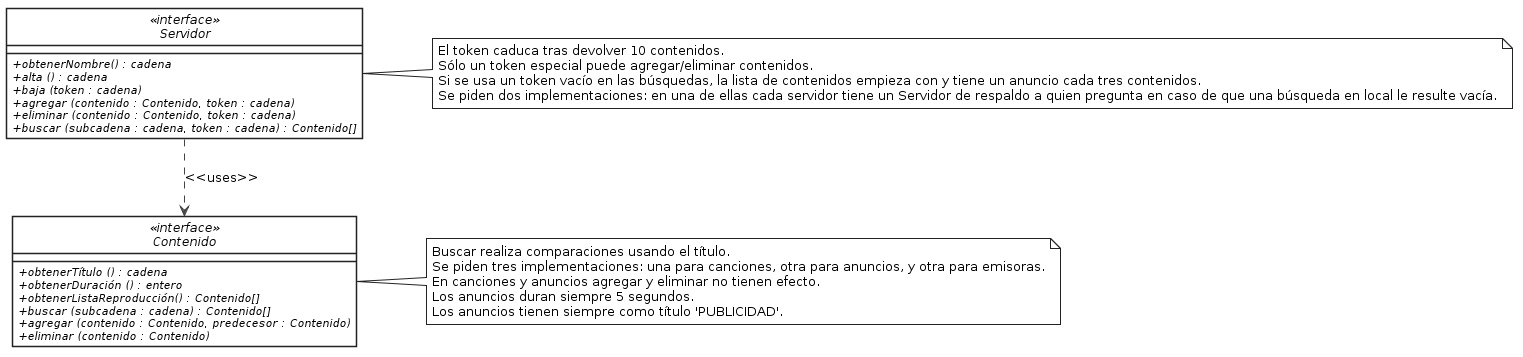
\includegraphics[width=18cm]{Imagenes/DiagramaSimple.png}\\
	A partir de dicho diagrama obtuvimos la siguiente relación de clases:\\
		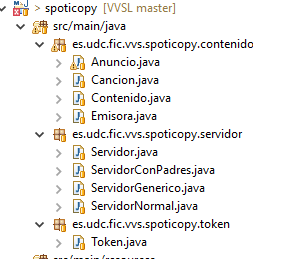
\includegraphics[width=8cm]{Imagenes/Clases.png} \\
	El paquete contenido tienen siempre un nombre, una duración y una lista de reproducción. Son las unidades funcionales con las que funcionará nuestro servidor.
	El paquete servidor es el que utiliza el paquete contenido para simular el funcionamiento de una aplicación que reproduce música. Distinguiremos ServidorGenerico que contiene el comportamiento genérico de un servidor. Las particularidades se implementan en distintas clases que heredaran de ServidorGenerico.
	El servidor normal simplemente implementa la búsqueda además de heredar del servidor genérico.
	La peculiaridad de un ServidorConPadres es que, de no poder devolver contenidos que cumplan el criterio de busqueda, solicita los contenidos de otro servidor, llamado padre, y devuelve lo que el le proporcione. Cualquier servidor puede ser el padre, no necesariamente otro Servidor ConPadres (aunque seria posible montarse arboles, listas o mallas de Servidores). OJO,la implementación no contempla el caso de un anillo de servidores, intentarlo creara un bucle infinito.

	
	\section{Estado actual}
	
	Listaxe de funcionalidades actuais, as súas especificacións, as persoas responsables do seu desenvolvemento, e as persoas responsables do proceso de proba.  Para cada funcionalidade: número de probas obxectivo, número de probas preparadas, porcentaxe executada e porcentaxe superada. Se esta información é profusa e se almacena noutra fonte, referencia á fonte. Se é cambiante, referencia a unha \emph{shapshot} ou resumo do mais destacado.\\ \\
	Las funciones que se ocupan de la funcionalidad de nuestra aplicación son las siguientes son las que serán evaluadas:
		\begin{itemize}
			\item Clase Anuncio
				\subitem String obtenerTitulo(): 
				\subitem int obtenerDuracion()
				\subitem List:Contenido obtenerListaReproduccion()
				\subitem List:Contenido buscar(final String subcadena)
				\subitem	void agregar(final Contenido contenido, final Contenido predecesor)
				\subitem	eliminar(final Contenido contenido)
			\item Clase Cancion
				\subitem String obtenerTitulo()
				\subitem int obtenerDuracion()
				\subitem List:Contenido obtenerListaReproduccion()
				\subitem List:Contenido buscar(final String subcadena)
				\subitem	void agregar(final Contenido contenido, final Contenido predecesor)
				\subitem	eliminar(final Contenido contenido)
			\item Clase Emisora
				\subitem String obtenerTitulo()
				\subitem int obtenerDuracion()
				\subitem List:Contenido obtenerListaReproduccion()
				\subitem List:Contenido buscar(final String subcadena)
				\subitem agregar(final Contenido contenido, final Contenido predecesor)
				\subitem eliminar(final Contenido contenido)
			\item Clase Token
				\subitem String alta()
				\subitem baja(final String token)
				\subitem boolean isAdminToken(final String token)
				\subitem long obtenerUsos(final String token)
				\subitem usarToken(final String token)
			\item Clase ServidorGenerico
				\subitem String obtenerNombre()
				\subitem List:Contenido getContenidos()
				\subitem Token getToken()
				\subitem String alta()
				\subitem baja(final String tok)
				\subitem agregar(final Contenido contenido, final String tok)
				\subitem eliminar(final Contenido contenido, final String tok)
			\item Clase ServidorNormal
				\subitem List:Contenido buscar(final String subcadena, final String tok)
			\item Clase ServidorConPadres
				\subitem List:Contenido buscar(final String subcadena, final String tok)
		\end{itemize}
	
	El objetivo es probar que todas estas funciones funcionan correctamente, para ello aplicaremos pruebas de unidad, pruebas dinámicas, pruebas de rendimiento y chequearemos el estilo de programación.
	Después de aplicarle las herramientas de pruebas y utilizar las herramientas de validación como cobertura y PIT creemos que nuestras funciones son estables y que puede que tengamos una bastantes pruebas realizadas y el código testeado para fiarnos de él. 
	
	\section{Registro de pruebas}
	\subsection{Pruebas unidad: JUnit}
	JUnit se utiliza para realizar pruebas unitarias sobre nuestra aplicación, nos sirven para encontrar errores y solventar los problemas en la programación de forma manual.
	Se realizan pruebas de todas las funciones implementadas en la aplicación.
	Los casos de prueba se implementan manualmente como parte de funciones de prueba, utilizamos la directiva assertEqual(Expected, Expr).
	\subsection{Pruebas basadas en propiedades: Quickcheck}
	QuickCheck es una  herramienta para generar automáticamente y ejecutar casos de prueba aleatorios, basados en especificaciones de propiedades. Es decir, ejecutar pruebas con esta herramienta, significa instanciar las propiedades n veces. Las pruebas se detienen al encontrar un caso concreto en el que la propiedad no se cumple
	(contraejemplo).La ejecución con éxito significa que ninguno de los casos generados incumplió la propiedad
	Se crean generadores de:
	\begin{itemize}
		\item GeneradorContenido
		\item GeneradorCancion
		\item GeneradorServidor
		\item GeneradorServidorVacio
	\end{itemize}
	
	La programación de generadores para aplicar Quickcheck se realiza en la siguiente clase: es.udc.fic.vvs.spoticopy.generadorTest.servidorTest. 
	
	\subsection{Validación de calidad de las pruebas: Cobertura}
	Cobertura( \href{http://cobertura.sourceforge.net/}{Plugin cobertura}) es una herramienta libre (GPL) escrita en Java, que nos permite comprobar el porcentaje de código al que accedemos desde los test. Es decir, Cobertura nos permite saber cuanto código estamos realmente probando con nuestros test.
	De esta forma Cobertura se convierte en una potente herramienta de trabajo, ya que lo podemos usar como medida de calidad (mientras más código tengamos probado, más garantías tenemos de que podemos hacer refactorizaciones sin peligro).
	Nuestro objetivo es llegar a cobertura cercana a 100.
	
	\subsection{Pruebas dinámicas de unidad: Mockito}
	Para poder crear un buen conjunto de pruebas unitarias, es necasario que nos centremos exclusivamente en la clase a testear, simulando el funcionamiento de las capas inferiores (pensad por ejemplo en olvidarnos de la capa de acceso a datos, DAO). De esta manera estaremos creando test unitarios potentes que os permitiría detectar y solucionar los errores que tengáis o que se cometan durante el futuro del desarrollo de vuestra aplicación.
	Para esta tarea nos apoyaremos en el uso de mock objects, que no son más que objetos que simulan parte del comportamiento de una clase, y más especificamente vamos a ver una herramienta que permite generar mock objects dinámicos, mockito.
	
	Pruebas que se realizarán en el paquete es.udc.fic.vvs.spoticopy.mockito, sólo se realizarán las pruebas del servidor, debido a que las pruebas de componentes ya son pruebas de unidad.
	\subsection{Pruebas no funcionales: JETM}
	JETM permite realizar pruebas de rendimiento y comprobar la velocidad de ejecuciones al implementar unas pruebas con n iteraciones. Se pueden generar test con múltiples iteraciones para detectar problemas de rendimiento.
	\subsection{Validación de calidad de las pruebas (mutación testing): PIT}
	
	El  método que utilizaban en el sistema para realizar estas mediciones lo denominaba “Programa mutado”.
	Básicamente, el Mutation testing consiste en introducir pequeñas modificaciones en el código fuente de la aplicación, a las que denominaremos mutaciones o mutantes.
	
	Si las pruebas pasan al ejecutarse sobre el mutante, el mutante sobrevive.
	Si las pruebas no pasan al ejecutarse sobre el mutante, el mutante muere
	El objetivo es que todos los mutantes mueran, así podremos decir que el test responde a la definición concreta del código y que lo prueba correctamente.
	Este concepto se basa en dos hipótesis:
	\begin{itemize}
	\item Hipótesis del programador competente: La mayoría de los errores introducidos por programadores Senior consisten en pequeños errores sintácticos.
	\item Hipótesis del efecto de acoplamiento: Pequeños fallos acoplados pueden dar lugar a otros problemas mayores.
		\end{itemize}
	Problemas de mayor orden serán revelados por mutantes de mayor orden, que se crean mediante la unión de multiples mutaciones.
	
		\subsection{Pruebas estructurales: CheckStyle}
		
		Checkstyle es una herramienta de desarrollo que ayudar a los programadores a escribir código Java para que se adhiera a un estándar de codificación. Automatiza el proceso de comprobación de código Java. Esto lo hace ideal para los proyectos a los que se desea aplicar un estándar de codificación.
		
		Checkstyle es altamente configurable y se puede hacer para apoyar casi cualquier estándar de codificación. De tal manera que se puedan suministrar diferentes estándares de código para su posterior comprobación mediante la herramienta.
		
		Reglas del CheckStyle
		El conjunto de reglas disponible es muy completo y está clasificado en los siguientes grupos:
	\begin{itemize}
		\item Comentarios Javadoc: facilitar el mantenimiento pasa por comentar el código, pero luego los comentarios también hay que mantenerlos... CheckStyle tiene muchas reglas para los javadoc y es muy flexible. Te permite, por ejemplo, obligar a comentar los nombres de clases, todos los métodos menos los get/set y los atributos públicos.
		\item Convenciones de nombres: puedes definir una expresión regular para el nombre de todo. 
		\item 	Cabeceras: expresiones regulares para la cabecera de los ficheros.
		\item Imports: reglas para los import, como no usar *, imports sin usar, etc.
		\item Violaciones de tamaño: define un máximo para el tamaño de tus clases, métodos, líneas y número de parámetros de un método.
		Espacios en blanco: un montón de reglas para definir donde se ponen espacios en blanco y tabuladores en el código.
		\item Modificadores: establece un orden para los modificadores y evita modificadores innecesarios.
		\item Bloques: reglas para los bloques de código y sus llaves.
		\item Problemas en la codificación: Acá hay de todo, desde malas prácticas tipo asignaciones internas y posibles fuentes de bugs como definir un método equals que no es el equals(Object), a cosas más estéticas o poco prolijas, como que el default sea el último elemento en un switch o paréntesis innecesarios.
		\item Diseño de clases: varias reglas sobre el diseño de interfaces y clases, con especial atención en las excepciones.
		\item Duplicados: te permite definir un mínimo de líneas para buscar código duplicado en tus clases.
		\item Métricas: define máximos para métricas como complejidad ciclomática, complejidad de expresiones lógicas, npath, líneas de código seguidas sin comentar y dependencia de clases.
		\item Misceláneo: variables final, indentación, un buscador de expresiones regulares y varias cosas más.
		\item J2EE: reglas para EJBs.
		\item Otros: internos a CheckStyle y activados por defecto.
		\item Filtros: para eventos de auditoria del propio CheckStyle, no hace falta mirarlos.
	\end{itemize}	
		Checkstyle es una herramienta de desarrollo para ayudar a los programadores escribir código Java que se adhiere a un estándar de codificación. 
		Para comprobar el estilo, pasamos la herramienta CheckStyle a nuestra aplicación y comprobamos el resultado:

		
	\section{Registro de errores}
	\subsection{Pruebas unidad: JUnit}
	En la primera iteración se encuentra que faltan test de funciones, se añaden los test que faltan y se comprueba q no fallan.
	
	Todos los errores localizados, modificaciones necesarias, etc. pueden encontrarse referenciados en el documento de CHANGELOG.txt, en el cual se encuentran las correcciones hasta el momento.
	
	\subsection{Validación de la calidad de las pruebas: Cobertura}
	Realizada la prueba de cobertura de pruebas, se observa que faltan muchos test por implementar, por lo que se procede a implementar los test que faltan, según la información que nos ofrece el plugin de ecobertura.\\
	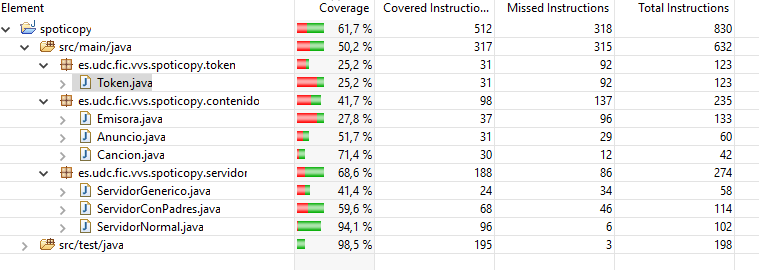
\includegraphics[width=15cm]{Imagenes/CoberturaSemana1.png} \\
	Después utilizar Junit y Quickcheck para:
	\begin{itemize}
		\item Aumentar cobertura de Anuncio (casi al 100%)
		\item Aumentar cobertura de ServidorNormal (al 100%)
		\item Aumentar cobertura de ServidorGenerico (casi al 100%)
		\item Aumentar cobertura de Token 
		\item Aumentar cobertura de ServidorConPadres
	\end{itemize}
	Quedó:
	
	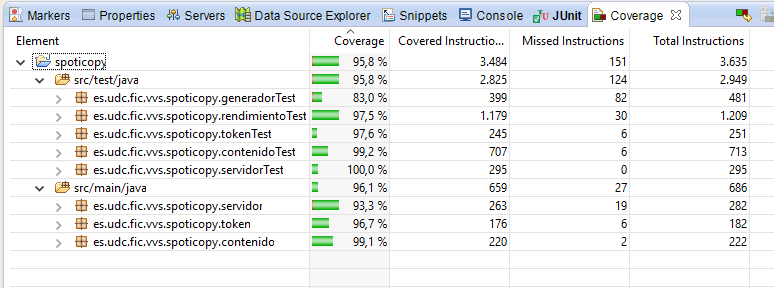
\includegraphics[width=15cm]{Imagenes/Covertura3.png}
	
	\subsection{Pruebas no funcionales: JETM}
	Resultado del rendimiento de JETM:
	href{Informes/SiteTestInicial/jetm-timing-report.html}{Informe JETM} \\
	
	
	\subsection{Validación de calidad de las pruebas (mutación testing): PIT}
	Realizado el mutation testing, resultados:
	
	\href{Informes/PIT1/index.html}{Informe PIT} \\
	
	\subsection{Pruebas estructurales: CheckStyle}
	Podemos comprobar los herrores encontrados en el siguiente informe: \href{Informes/SiteTestInicial/checkstyle.html}{Informe CheckStyle} \\
	Al pasar la herramienta de CheckStyle descubrimos que nuestra aplicación tiene unos 236 errores de estilo, es decir, que no cumple el estandar de programación java.
	
	Resumen de errores encontrados:
	\begin{itemize}
		\item Faltan comentarios: En la mayoría de clases faltan comentarios javadoc. Se añaden.
		\item Mala indexación código y espacios: Se reestructura el código para que solventar dichos errores.
		\end{itemize}
		
		Se revisa el informe con los 236 errores de estilo y se eliminan los 236 errores de estilo.
		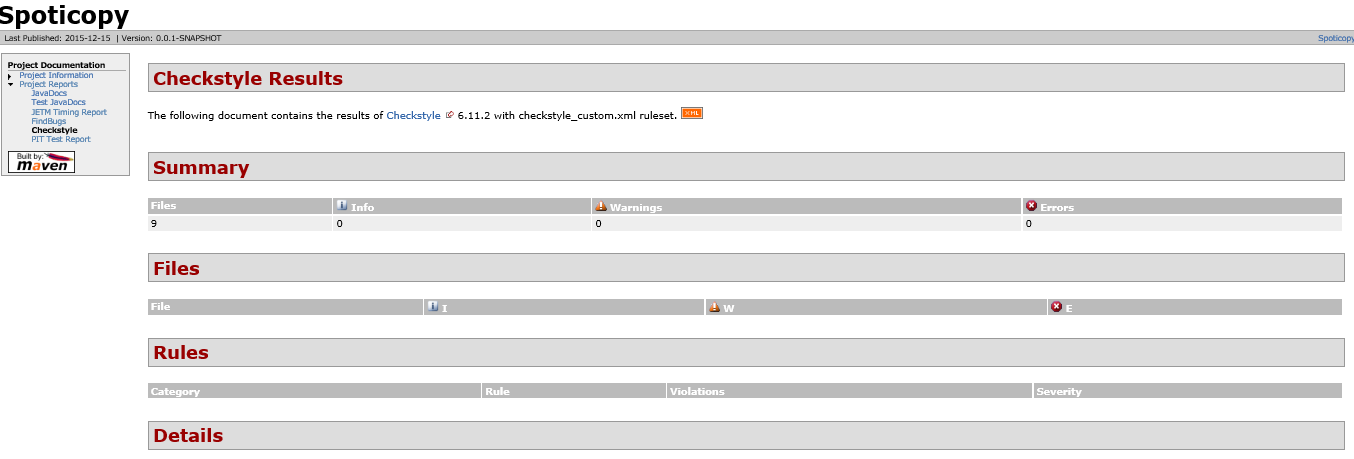
\includegraphics[width=15cm]{Imagenes/CheckStyleResut.png} \\
	\subsection{Pruebas estáticas/estructurales: FindBugs}
	
	FindBugs es un programa que utiliza el análisis estático para buscar errores en el código de Java.
	
	En la versión inicial podemos comprobar que tenemos los siguientes errores:
	\href{Informes/SiteTestInicial/findbugs.html}{Informe Find bugs} \\

	Errores encontrados:
	\begin{itemize}
		\item 	ST WRITE TO STATIC FROM INSTANCE METHOD: En la clase token existía un método que escribía en una variable estática, esto es una mala práctica cuando está siendo manipulado por varias instancias.
		\item 	RI REDUNDANT INTERFACES: ServidorNormal y ServidorConPadres implementa la misma interfaz que la superclase.
		\item BC EQUALS METHOD SHOULD WORK FOR ALL OBJECTS: El método equals (Object o) no debe hacer ninguna suposición sobre el tipo de o. Simplemente debe devolver false si o no es del mismo tipo que esta. La clase Anuncio asume el argumento es de tipo anuncio.
		\item HE EQUALS USE HASHCODE: La clase anuncio Esta clase anula Equals (Object) , pero no anula hashCode () , y hereda la implementación de hashCode () de java.lang.Object (que devuelve el código hash de identidad, un valor arbitrario asignado al objeto por el VM ) . Por lo tanto , es muy probable que violaría el invariante que los objetos iguales deben tener iguales hashcodes la clase.
		\item NP EQUALS SHOULD HANDLE NULL ARGUMENT: En la clase anuncio, el método no funciona para cuando el objeto es nulo.	
	\end{itemize}
	Después de identificar los errores, resolvedos los problemas mencionados y comprobamos el resultado:\\
	\\
	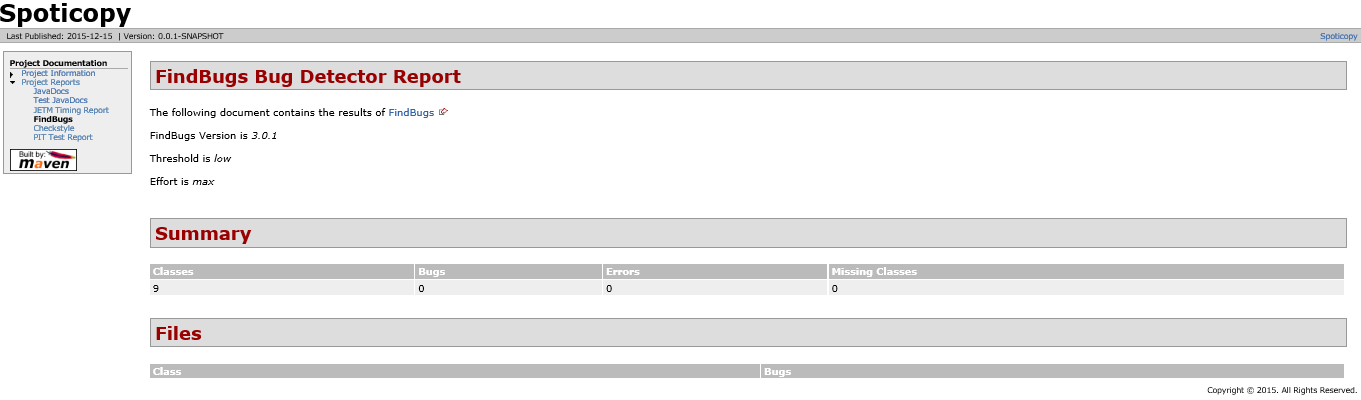
\includegraphics[width=15cm]{Imagenes/FindsBugs2.png} \\

	\section{Otros aspectos de interés}
	
	Nada de momento. Se conserva el apartado para el futuro.
	
\end{document}